\ylDisplay{Miku ja kärbes} % Ülesande nimi
{Tundmatu autor} % Autor
{piirkonnavoor} % Voor
{2003} % Aasta
{P 5} % Ülesande nr.
{2} % Raskustase
{
% Teema: Valgusõpetus
\ifStatement
Toa seinal on $1$ m laiune peegel. Miku seisab toas näoga seina poole, $3$ m kaugusel seinast ja $2$ m kaugusel peegli keskristsirgest. Akki näeb Miku peegli servas peeglist eemale lendava kärbse kujutist. Kui kiiresti peaks Miku taganema peegliga seinast eemale, et näha kogu 1 oma liikumise aja jooksul kärbse kujutist peegli servas, kui kärbes lendab piki peegli pinna keskristsirget peeglist eemale kiirusega $0,5$ m/s?
\begin{center}
	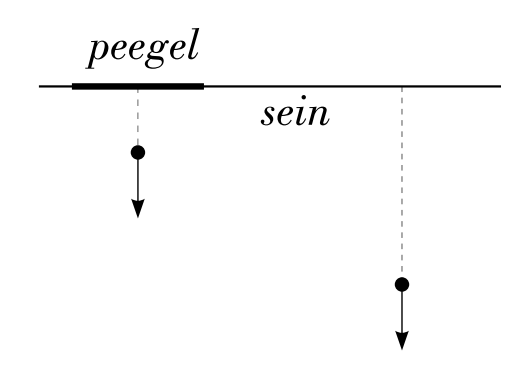
\includegraphics[width=0.5\linewidth]{2003-v2p-05-yl.PNG}
\end{center}
\fi

\ifHint
Ülesande lahendamisel tuleb konstrueerida joonis ning kasutada peegeldumise seadust ning kolmnurkade sarnasusi.
\fi


\ifSolution
Kasutame peegeldumise seadust, kolmnurkade $BA'C$ ja $CDE$ sarnasust ja kolmnurkade $BA'C$ ja $BAC$ võrdsust. Selgub, et Miku, kes on $3 m$ kaugusel seinast ja $1,5 m$ kaugusel peegli servast, näeb kärbse kujutist siis, kui kärbes on peeglist $1 m$ kaugusel. Arvestades kärbse kiirust, leiame Miku kauguse seinast näiteks $1 s$ pärast $(4,5 m)$. Miku liikumise kiirus on seega $4,5 m - 3 m/1 s= 1$, $5$ m/s.
\begin{center}
	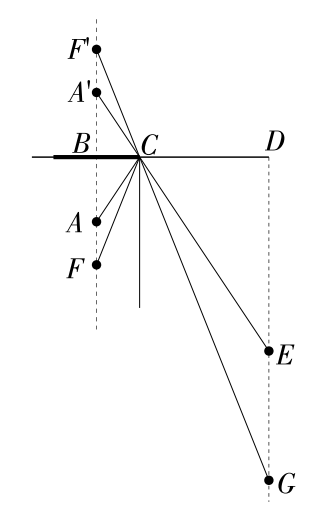
\includegraphics[width=0.5\linewidth]{2003-v2p-05-lah.PNG}
\end{center}
\fi
}
 
